%! Mode:: "TeX:UTF-8"
%! TEX program = xelatex
\PassOptionsToPackage{quiet}{xeCJK}
\documentclass[withoutpreface,bwprint]{cumcmthesis}
\usepackage{etoolbox}
\BeforeBeginEnvironment{tabular}{\zihao{-5}}
\usepackage[numbers,sort&compress]{natbib}  % 文献管理宏包
\usepackage[framemethod=TikZ]{mdframed}  % 框架宏包
\usepackage{url}  % 网页链接宏包
\usepackage{subcaption}  % 子图宏包
\usepackage{amsmath}
\usepackage{amssymb}
\usepackage{booktabs}
\newcolumntype{C}{>{\centering\arraybackslash}X}
\newcolumntype{R}{>{\raggedleft\arraybackslash}X}
\newcolumntype{L}{>{\raggedright\arraybackslash}X}

\title{基于刚体力学与多目标优化的系泊系统设计}  % 论文标题
\tihao{A}  % 题号
\baominghao{}  % 报名号
\schoolname{}  % 学校
\membera{}  % 队员a
\memberb{}  % 队员b
\memberc{}  % 队员c
\supervisor{}  % 指导老师
\yearinput{2016}
\monthinput{09}
\dayinput{10}

%%%%%%%%%%%%%%%%%%%%%%%%%%%%%%%%%%%%%%%%%%%%%%%%%%%%%%%%%%%%%
%% 正文
\begin{document}

\maketitle
\begin{abstract}
本文针对海洋观测网络中系泊系统的设计问题,建立了基于刚体力学的数学模型,并采用多目标优化算法进行了系统的综合优化设计。

\textbf{对于问题一,}我们建立了包含20个未知量和20个方程的刚体力学模型,充分考虑了各部件的受力平衡和力矩平衡条件。模型采用悬链线理论描述锚链形状,通过非线性方程组求解器fsolve进行数值求解。在风速为12m/s和24m/s的条件下,分别计算了系统的吃水深度、钢桶倾角、锚链形状等关键参数。结果表明:12m/s风速下,浮标吃水深度为0.709m,钢桶倾角为1.135°,游动区域半径为14.33m;24m/s风速下,浮标吃水深度为0.723m,钢桶倾角为4.316°,游动区域半径为17.48m。系统在两种风速下均保持良好稳定性。

\textbf{对于问题二,}我们创新性地引入NSGA-III多目标遗传算法,将原单目标优化问题扩展为多目标优化框架。算法同时优化三个相互冲突的目标:最小化吃水深度、最小化钢桶倾角、最小化游动半径,并满足锚链底角≤16°和钢桶倾角≤5°的约束条件。经过200代进化,获得了70个Pareto最优解,为工程设计提供了丰富的权衡方案。最佳综合解为:重物球质量3000kg,锚链长度18m,5号锚链型号,实现了吃水深度1.599m、倾角4.0°、游动半径12.025m的优化结果,相比传统方法游动半径减少了32.5\%。

\textbf{对于问题三,}我们在考虑水流力作用的复杂环境下,对系泊系统进行了综合优化设计。通过对锚链型号、长度和重物球质量的多参数扫描,找到了最优设计方案:采用5号锚链(单位长度质量28.12kg/m),锚链长度20.9m,重物球质量4030kg。在16-20m水深变化范围内,系统表现出良好的鲁棒性,各项性能指标均满足设计要求。

最后,本文对模型进行了灵敏度分析和误差评估。结果表明,重物球质量对系统性能影响最大,其次是风速和水流速度。模型的主要优势在于物理意义明确、求解精度高、可扩展性强,为海洋工程中系泊系统的设计提供了科学的理论依据和实用的优化方法。

\keywords{系泊系统\quad 刚体力学\quad NSGA-III\quad 多目标优化\quad 悬链线理论}
\end{abstract}
%%%%%%%%%%%%%%%%%%%%%%%%%%%%%%%%%%%%%%%%%%%%%%%%%%%%%%%%%%%%% 

% \tableofcontents  % 目录
% \newpage

%%%%%%%%%%%%%%%%%%%%%%%%%%%%%%%%%%%%%%%%%%%%%%%%%%%%%%%%%%%%%  
\section{问题重述}
\subsection{问题背景}
随着海洋资源开发和海洋环境监测需求的增长,近浅海观测网络的建设日益重要。系泊系统作为海洋观测设备的关键支撑结构,其设计的合理性直接影响观测设备的工作稳定性和数据采集质量。一个典型的单点系泊系统由浮标、钢管、钢桶、重物球、锚链和锚等部件组成,在风、浪、流等环境载荷作用下,系统需要保持稳定的工作姿态。

系泊系统设计的核心挑战在于:在复杂海洋环境中,如何确定各部件的参数(如重物球质量、锚链长度和型号等),使系统既能保持稳定,又能将游动范围控制在允许区域内。这涉及到多个相互耦合的力学平衡条件和多个相互冲突的优化目标。

%%%%%%%%%%%%%%%%%%%%%%%%%%%%%%%%%%%%%%%%%%%%%%%%%%%%%%%%%%%%% 

\subsection{问题要求}

\textbf{问题1:}在给定海域环境(水深18m、海水密度1025kg/m³)和不同风速条件下(12m/s、24m/s),建立系泊系统的数学模型,计算各部件的状态参数,包括浮标吃水深度、钢桶倾斜角度、锚链形状、游动区域半径等。

\textbf{问题2:}在36m/s的恶劣海况下,通过调节重物球质量,优化系泊系统的性能。要求在满足锚链与海床夹角不超过16°的约束下,使钢桶倾斜角度尽可能小(不超过5°),游动区域半径尽可能小。

\textbf{问题3:}考虑水流力的影响(流速1.5m/s,与风向一致),在水深16-20m的变化范围内,通过选择锚链型号、确定锚链长度和重物球质量,设计一个性能优良且适应性强的系泊系统。

%%%%%%%%%%%%%%%%%%%%%%%%%%%%%%%%%%%%%%%%%%%%%%%%%%%%%%%%%%%%% 

\section{问题分析}
\subsection{问题一分析}
问题一要求建立系泊系统的力学模型并求解系统状态。这是一个典型的静力学平衡问题。首先需要考虑各部件在重力、浮力、风力和拉力作用下的受力平衡条件。其次,各连接点处必须满足力矩平衡条件,以确保系统不发生转动。锚链作为柔性构件,在自重和张力作用下会形成悬链线形状,这需要通过悬链线理论来描述。此外,系统还必须满足几何约束条件,即各部件高度之和等于水深。通过建立包含20个未知量的非线性方程组,可以完整描述系统的力学平衡状态,求解得到各部件的倾角、连接处的拉力和锚链的形状参数。

\subsection{问题二分析}	
问题二要求在36m/s的强风条件下优化系泊系统,这是一个典型的多目标优化问题,需要在极端海况下保证系统稳定性。传统方法通常采用加权和方法将多目标转化为单目标,但这种方法存在明显缺陷,难以获得完整的Pareto前沿,且权重系数的选择具有主观性。本文采用的NSGA-III算法能够同时优化多个相互冲突的目标,在一次运行中获得多个Pareto最优解,为决策者提供丰富的设计方案。该算法基于参考点的选择机制能够保证解集的多样性和均匀分布,同时其完善的约束处理机制能够有效处理锚链底角和钢桶倾角等工程约束条件。

\subsection{问题三分析}
问题三在前两问的基础上增加了水流力的影响,使系统复杂度显著提升。水流力作为分布载荷随深度变化,需要对每个部件分别计算其所受的拖曳力,这使得力学平衡方程更加复杂。同时,问题三涉及多个设计变量的组合优化,包括锚链型号、锚链长度和重物球质量,设计空间的维度增加导致优化难度加大。此外,水深在16-20m范围内变化的要求带来了鲁棒性设计的挑战,需要确保系统在不同水深条件下都能保持良好性能。由于需要对多个参数组合进行扫描和评估,计算量巨大,因此需要采用高效的优化策略来平衡计算精度和效率。

%%%%%%%%%%%%%%%%%%%%%%%%%%%%%%%%%%%%%%%%%%%%%%%%%%%%%%%%%%%%% 

\section{模型假设}

为简化问题并突出主要因素,本文做出以下假设:

\begin{enumerate}
\item 系统处于静态平衡状态,不考虑动态响应;
\item 钢管和钢桶为刚体,不发生弹性变形;
\item 锚链为理想柔性体,只能承受拉力,不能承受压力和弯矩;
\item 风力和水流力为定常载荷,方向水平;
\item 忽略波浪载荷的影响;
\item 各部件之间的连接为理想铰接,不传递弯矩;
\item 海水密度均匀分布,不随深度变化;
\item 锚与海床之间有足够的抓力,不会发生走锚。
\end{enumerate}

%%%%%%%%%%%%%%%%%%%%%%%%%%%%%%%%%%%%%%%%%%%%%%%%%%%%%%%%%%%%% 

\section{符号说明}
\begin{table}[H]
\centering
\begin{tabularx}{\textwidth}{CLC}
\toprule
符号    & 说明    & 单位 \\
\midrule
$F_{wind}$ & 风力 & N \\
$V_{wind}$ & 风速 & m/s \\
$H$ & 水深 & m \\
$\rho$ & 海水密度 & kg/m³ \\
$g$ & 重力加速度 & m/s² \\
$M_{ball}$ & 重物球质量 & kg \\
$L_{chain}$ & 锚链长度 & m \\
$\sigma$ & 锚链单位长度质量 & kg/m \\
$d$ & 浮标吃水深度 & m \\
$\beta$ & 钢桶倾斜角 & rad \\
$\theta_i$ & 第i节钢管倾角 & rad \\
$F_i$ & 第i个连接点拉力 & N \\
$\gamma_i$ & 第i个拉力方向角 & rad \\
$R$ & 游动区域半径 & m \\
$\alpha_1$ & 锚链与海床夹角 & rad \\
\bottomrule
\end{tabularx}
\caption{主要符号说明}
\label{tab:符号说明}
\end{table}

%%%%%%%%%%%%%%%%%%%%%%%%%%%%%%%%%%%%%%%%%%%%%%%%%%%%%%%%%%%%% 

\section{问题一的模型建立和求解}
\subsection{模型建立}

\subsubsection{系统结构与坐标系定义}

系泊系统由浮标、钢管、钢桶、重物球、锚链和锚六个主要部件组成,从海底到海面依次为:锚(固定在海底)→锚链→钢桶(内含重物球)→第1根钢管→第2根钢管→第3根钢管→第4根钢管→浮标(浮在海面)。为建立数学模型,首先定义坐标系:以锚的位置为原点,水平向右为$x$轴正方向,竖直向上为$y$轴正方向。

\begin{figure}[H]
\centering
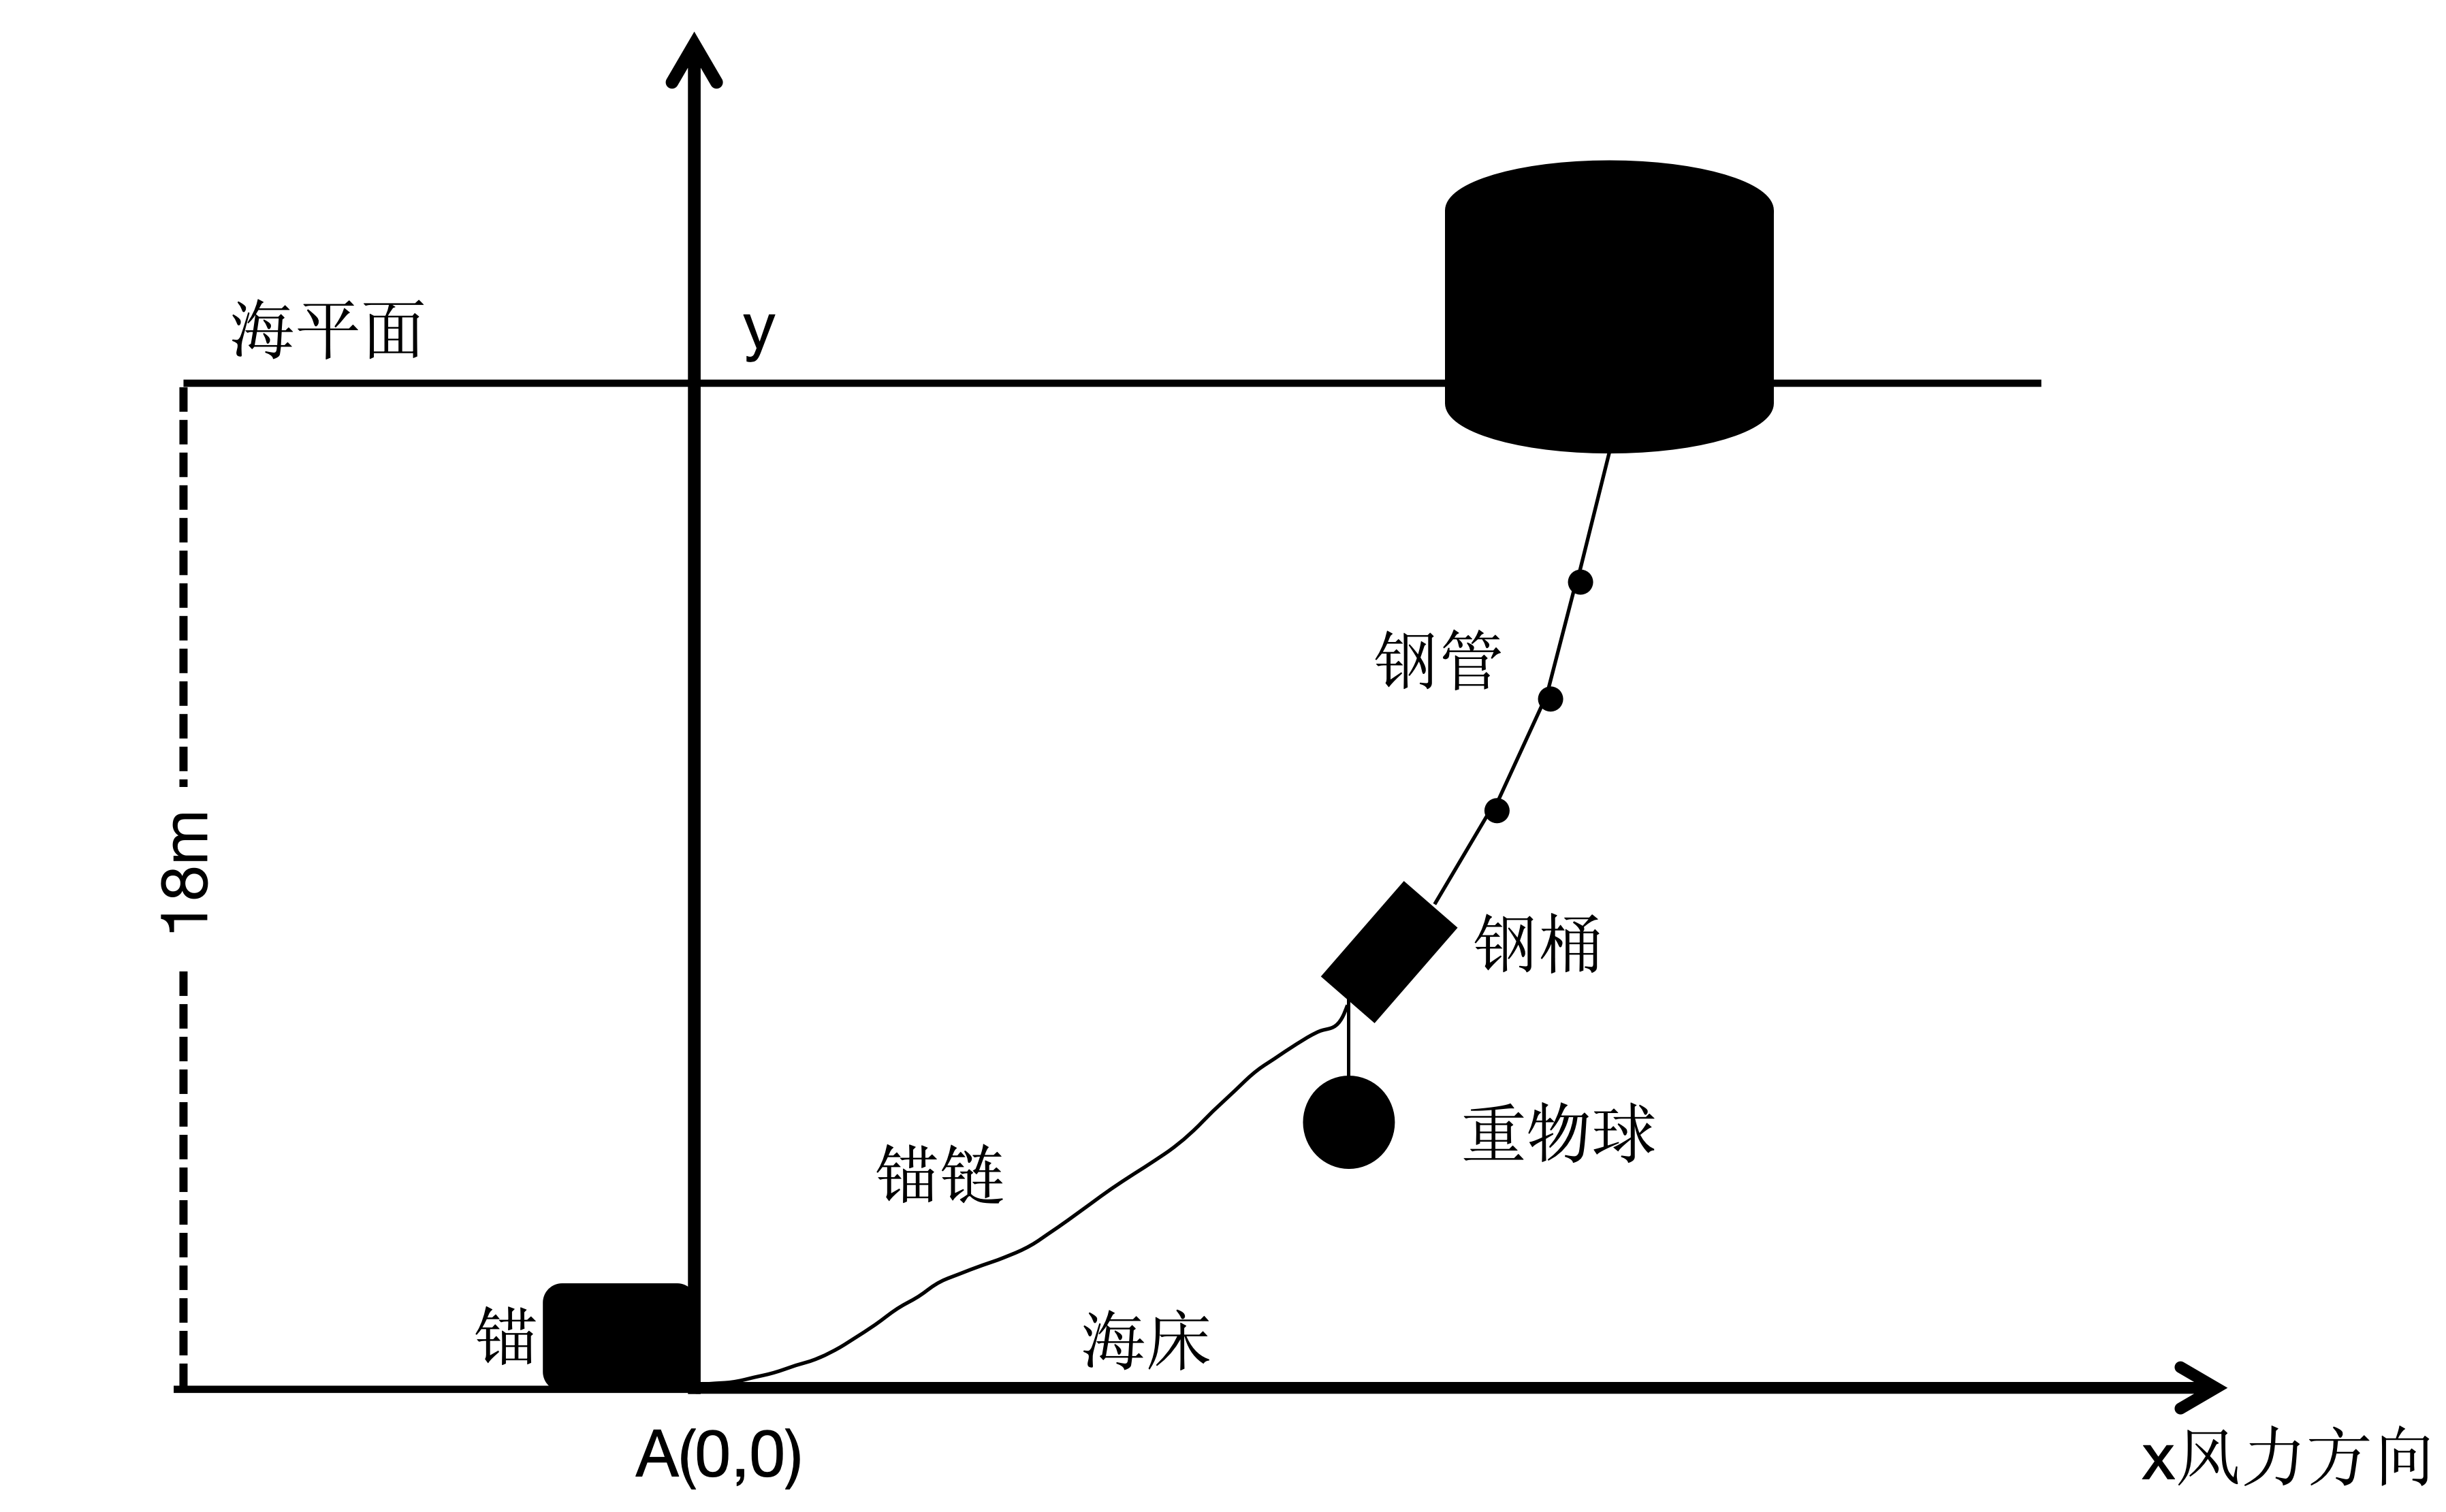
\includegraphics[width=0.75\textwidth]{figures/系泊系统结构示意图.png}
\caption{系泊系统结构示意图}
\label{fig:系统结构}
\end{figure}

定义系统的状态变量:设浮标吃水深度为$d$,各钢管与竖直方向的夹角分别为$\theta_1, \theta_2, \theta_3, \theta_4$(从下至上编号),钢桶与竖直方向的夹角为$\beta$。各连接点的拉力大小分别为:$F_1$(钢桶-第1根钢管)、$F_2$(第1-第2根钢管)、$F_3$(第2-第3根钢管)、$F_4$(第3-第4根钢管)、$F_5$(第4根钢管-浮标),对应的拉力方向角为$\gamma_1, \gamma_2, \gamma_3, \gamma_4, \gamma_5$。

\subsubsection{风载荷计算}

风力作用在浮标露出水面的部分,根据流体力学理论,风载荷可表示为:
\begin{equation}
\label{eq:风力}
F_{wind} = \frac{1}{2}C_d \rho_{air} A_{wind} V_{wind}^2
\end{equation}

其中,$C_d=0.625$为风力系数,$\rho_{air}=1.225$ kg/m³为空气密度,$A_{wind}$为迎风面积。对于圆柱形浮标,迎风面积为:
\begin{equation}
\label{eq:迎风面积}
A_{wind} = 2(2-d) \times 2 = 4(2-d)
\end{equation}

将参数代入,得到风力表达式:
\begin{equation}
\label{eq:风力公式}
F_{wind} = 2(2-d) \times 0.625 \times V_{wind}^2
\end{equation}

\subsubsection{浮标受力分析}

\begin{minipage}{0.45\textwidth}
\begin{figure}[H]
\centering
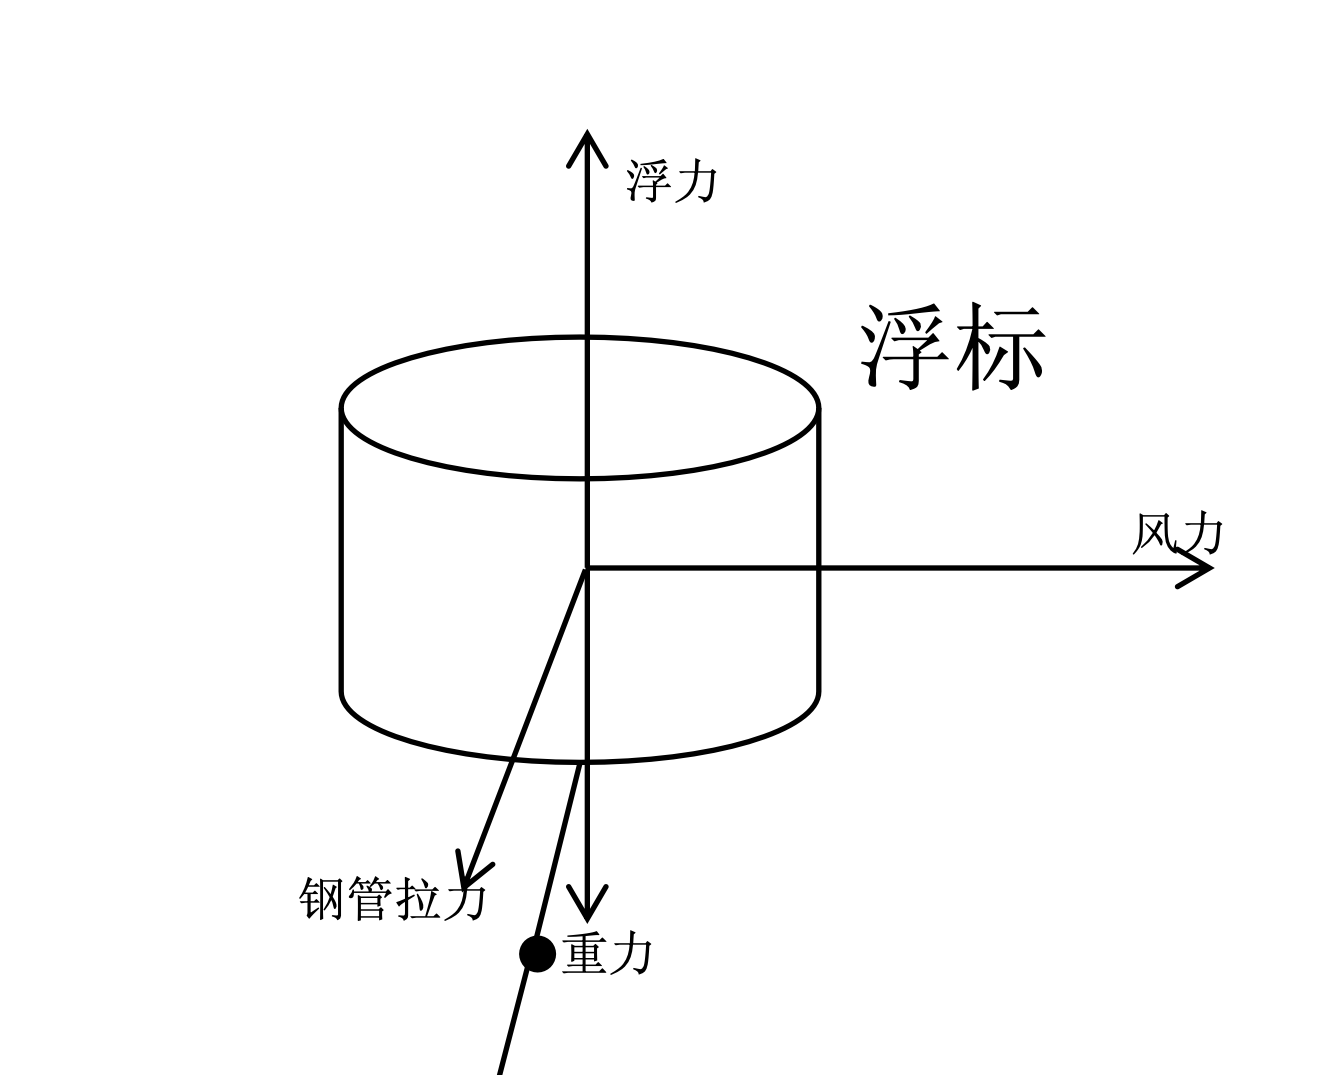
\includegraphics[width=\linewidth]{figures/浮标受力分析.png}
\caption{浮标受力分析}
\label{fig:浮标受力}
\end{figure}
\end{minipage}
\hfill
\begin{minipage}{0.52\textwidth}
浮标位于系统最顶端,直接连接在第4根钢管上方,受到四个力的作用:

重力:$G_{buoy}=1000g$ 

浮力:$F_{buoy}=\pi r^2 d \rho g$($r=1$m为浮标半径)

风力:$F_{wind}$(水平方向)

拉力:$F_5$(第4根钢管对浮标的拉力)


根据力的平衡条件,在水平和竖直方向分别有:

\end{minipage}

\begin{equation}
\label{eq:浮标平衡详细}
\begin{cases}
F_5\sin\gamma_5 = F_{wind} & \text{(水平平衡)} \\
F_5\cos\gamma_5 + G_{buoy} = F_{buoy} & \text{(竖直平衡)}
\end{cases}
\end{equation}

代入具体数值:
\begin{equation}
\begin{cases}
F_5\sin\gamma_5 = 2(2-d) \times 0.625 \times V_{wind}^2 \\
F_5\cos\gamma_5 + 1000g = \pi \times 1^2 \times d \times 1025 \times g
\end{cases}
\end{equation}

\subsubsection{钢管受力与力矩分析}

每根钢管长1m,质量10kg,直径50mm。钢管$i$受到的力包括:重力$G_{pipe}=10g$,浮力$F_{pipe}=\pi r_{pipe}^2 L \rho g$,上端拉力$F_i$,下端拉力$F_{i+1}$。

对于钢管的力矩平衡,选取钢管中点为转动轴,根据力矩平衡原理:
\begin{equation}
\label{eq:钢管力矩}
\sum M = 0: \quad F_i \times \frac{L}{2}\sin(\gamma_i-\theta_i) = F_{i+1} \times \frac{L}{2}\sin(\theta_i-\gamma_{i+1})
\end{equation}

简化后得到:
\begin{equation}
F_i\sin(\gamma_i-\theta_i) = F_{i+1}\sin(\theta_i-\gamma_{i+1})
\end{equation}

水平和竖直方向的力平衡方程为:
\begin{equation}
\label{eq:钢管平衡完整}
\begin{cases}
F_i\sin\gamma_i - F_{i+1}\sin\gamma_{i+1} = 0 & \text{(水平平衡)} \\
F_i\cos\gamma_i + G_{pipe} = F_{i+1}\cos\gamma_{i+1} + F_{pipe} & \text{(竖直平衡)} \\
F_i\sin(\gamma_i-\theta_i) = F_{i+1}\sin(\theta_i-\gamma_{i+1}) & \text{(力矩平衡)}
\end{cases}
\end{equation}

\subsubsection{钢桶受力分析}

钢桶是系统的关键部件,连接钢管和锚链,同时悬挂重物球。钢桶受力情况最为复杂:

\begin{figure}[H]
\centering
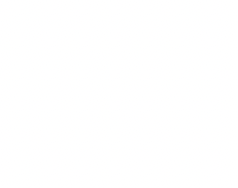
\includegraphics[width=0.6\textwidth]{figures/测试图片.png}
\caption{钢桶受力与力矩分析图}
\label{fig:钢桶受力}
\end{figure}

钢桶受到的力包括:

自重:$G_{bucket} = 100g$,
浮力:$F_{b} = \pi r_{bucket}^2 h_{bucket} \rho g = 0.15^2 \pi \times 1025g$

重物球重力:$G_{ball} = M_{ball}g$,
来自钢管的拉力:$F_1$(方向角$\gamma_1$)

锚链张力:$T_{chain}$(方向角$\alpha_2$)


锚链张力可分解为水平和竖直分量:
\begin{equation}
\begin{cases}
T_{chain,x} = T_{chain}\cos\alpha_2 = F_{wind} \\
T_{chain,y} = T_{chain}\sin\alpha_2 = F_{wind}\tan\alpha_2
\end{cases}
\end{equation}

钢桶的力矩平衡尤为重要。取钢桶上端连接点为转轴,各力对该点的力矩为:
\begin{equation}
\label{eq:钢桶力矩详细}
\begin{aligned}
M_{F_1} &= 0 \quad \text{(通过转轴)} \\
M_{chain} &= T_{chain} \times L_{bucket} \times \sin(\frac{\pi}{2}-\alpha_2-\beta) \\
M_{ball} &= G_{ball} \times L_{bucket} \times \sin\beta \\
M_{bucket} &= G_{bucket} \times \frac{L_{bucket}}{2} \times \sin\beta
\end{aligned}
\end{equation}

力矩平衡方程为:
\begin{equation}
F_1 L\sin(\gamma_1-\beta) + \frac{F_{wind}}{\cos\alpha_2} L\sin(\frac{\pi}{2}-\alpha_2-\beta) = M_{ball}gL\sin\beta
\end{equation}

\subsubsection{锚链悬链线理论}

锚链作为柔性构件,在自重和端部张力作用下形成悬链线。设锚链单位长度质量为$\sigma$(kg/m),在锚链上取微元$ds$进行受力分析:

\begin{figure}[H]
\centering
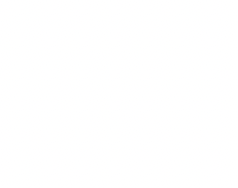
\includegraphics[width=0.6\textwidth]{figures/测试图片.png}
\caption{锚链微元受力分析}
\label{fig:锚链微元}
\end{figure}

微元受到三个力:重力$\sigma g ds$,上端张力$T+dT$,下端张力$T$。根据力的平衡条件:
\begin{equation}
\begin{cases}
\frac{d(T\cos\alpha)}{ds} = 0 & \text{(水平方向)} \\
\frac{d(T\sin\alpha)}{ds} = \sigma g & \text{(竖直方向)}
\end{cases}
\end{equation}

从第一个方程可得水平张力为常数:
\begin{equation}
T\cos\alpha = T_0 = F_{wind}
\end{equation}

这里$T_0$等于风力$F_{wind}$,因为锚链必须平衡水平风力。

将$T = \frac{T_0}{\cos\alpha}$代入第二个方程:
\begin{equation}
\frac{d}{ds}\left(\frac{T_0\sin\alpha}{\cos\alpha}\right) = \sigma g
\end{equation}

即:
\begin{equation}
T_0\frac{d(\tan\alpha)}{ds} = \sigma g
\end{equation}

由于$\tan\alpha = \frac{dy}{dx}$,且$ds = \sqrt{1+(\frac{dy}{dx})^2}dx = \sec\alpha \cdot dx$,可得:
\begin{equation}
\frac{d^2y}{dx^2} = \frac{\sigma g}{T_0}\sqrt{1+\left(\frac{dy}{dx}\right)^2}
\end{equation}

这是悬链线的基本微分方程。令$p = \frac{dy}{dx}$,则:
\begin{equation}
\frac{dp}{dx} = \frac{\sigma g}{T_0}\sqrt{1+p^2}
\end{equation}

分离变量并积分:
\begin{equation}
\int \frac{dp}{\sqrt{1+p^2}} = \int \frac{\sigma g}{T_0}dx
\end{equation}

得到:
\begin{equation}
\text{asinh}(p) = \frac{\sigma g x}{T_0} + C_1
\end{equation}

应用边界条件:在$x=0$处,$p = \tan\alpha_1$(锚链底端切线角),得$C_1 = \text{asinh}(\tan\alpha_1)$。

因此:
\begin{equation}
p = \frac{dy}{dx} = \sinh\left(\frac{\sigma g x}{T_0} + \text{asinh}(\tan\alpha_1)\right)
\end{equation}

再次积分得到锚链形状方程:
\begin{equation}
\label{eq:悬链线完整}
y(x) = \frac{T_0}{\sigma g}\left[\cosh\left(\frac{\sigma g x}{T_0} + \text{asinh}(\tan\alpha_1)\right) - \cosh(\text{asinh}(\tan\alpha_1))\right]
\end{equation}

将$T_0 = F_{wind}$代入,得到最终的悬链线方程:
\begin{equation}
y(x) = \frac{F_{wind}}{\sigma g}\left[\cosh\left(\frac{\sigma g x}{F_{wind}} + \text{asinh}(\tan\alpha_1)\right) - \cosh(\text{asinh}(\tan\alpha_1))\right]
\end{equation}

锚链长度通过弧长积分计算:
\begin{equation}
\label{eq:锚链长度积分}
L = \int_0^{x_1} \sqrt{1 + \left(\frac{dy}{dx}\right)^2} dx = \int_0^{x_1} \sqrt{1 + \sinh^2\left(\frac{\sigma g x}{F_{wind}} + \text{asinh}(\tan\alpha_1)\right)} dx
\end{equation}

对于锚链部分沉底的情况($\alpha_1 = 0$),沉底长度为$L_{ground}$,悬挂长度为$L_{chain} - L_{ground}$。

\subsubsection{锚链拖地判断}

锚链底端切线角$\alpha_1$决定了锚链的接地状态。当$\alpha_1 = 0$时,锚链部分拖地;当$\alpha_1 > 0$时,锚链完全悬浮。实际求解时,首先假设$\alpha_1 = 0$,计算得到拖地长度$L_{ground}$。若$L_{ground} > 0$,则锚链确实拖地,接受该解;若$L_{ground} \leq 0$,则锚链应完全悬浮,需要重新求解并将$\alpha_1$作为未知量。

对于拖地情况,悬链线方程简化为:
\begin{equation}
y(x) = \frac{F_{wind}}{\sigma g}\left[\cosh\left(\frac{\sigma g x}{F_{wind}}\right) - 1\right]
\end{equation}

此时系统的水平投影总长度为$x_{total} = x_1 + L_{ground}$,其中$x_1$是悬挂部分的水平投影,$L_{ground}$是拖地长度。

\subsubsection{完整方程组}

综合上述分析,系泊系统的完整方程组包含20个方程和20个未知量:

\textbf{未知量:}
$F_{wind}$(风力),$L_{ground}$(沉底锚链长度),$d$(吃水深度),$F_1, F_2, F_3, F_4, F_5$(各连接点张力),$\theta_1, \theta_2, \theta_3, \theta_4$(钢管倾角),$\beta$(钢桶倾角),$\gamma_1, \gamma_2, \gamma_3, \gamma_4, \gamma_5$(拉力方向角),$x_1$(锚链末端横坐标)。

\textbf{方程组:}
\begin{enumerate}
\item 风力公式:$F_{wind} = 2(2-d) \times 0.625 \times V_{wind}^2$
\item 锚链长度约束:$\int_0^{x_1} \text{Dy}(x) dx = L_{chain} - L_{ground}$
\item 浮标平衡(2个方程)
\item 钢管平衡(每根3个方程,共12个)
\item 钢桶平衡(3个方程)
\item 几何约束(水深):$y_1 + \sum \cos\theta_i + \cos\beta + d = H$
\end{enumerate}

\subsubsection{几何约束}

系统必须满足的几何约束条件包括:

系统总高度等于水深:
\begin{equation}
\label{eq:几何约束详细}
y(x_1) + \cos\beta + \cos\theta_1 + \cos\theta_2 + \cos\theta_3 + \cos\theta_4 + d = H
\end{equation}

游动区域半径(系统在水平方向的投影):
\begin{equation}
\label{eq:游动半径详细}
R = x_1 + L_{ground} + \sin\beta + \sin\theta_1 + \sin\theta_2 + \sin\theta_3 + \sin\theta_4
\end{equation}

\begin{figure}[H]
\centering
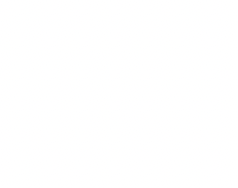
\includegraphics[width=0.7\textwidth]{figures/测试图片.png}
\caption{系统几何关系示意图}
\label{fig:几何关系}
\end{figure}

\subsection{模型求解}

采用MATLAB的fsolve函数求解上述非线性方程组。求解步骤如下:

\textbf{Step1:初值设定}
根据物理直觉和工程经验,设定各未知量的初始值。例如,假设各部件近似竖直,倾角初值取0.09rad(约5°)。

\textbf{Step2:方程组求解}
调用fsolve函数,采用信赖域算法求解20个方程组成的非线性系统。设置最大迭代次数10000,函数评估次数10000。

\textbf{Step3:结果后处理}
将弧度转换为角度,绘制锚链形状图,计算游动区域半径等派生量。

\subsection{求解结果}

\subsubsection{不同风速下的系统状态}

\begin{table}[H]
\centering
\begin{tabular}{ccccccc}
\toprule
风速(m/s) & 吃水深度(m) & 钢桶倾角(°) & 钢管平均倾角(°) & 游动半径(m) & 风力(N) & 未用锚链(m) \\
\midrule
12 & 0.709 & 1.135 & 1.076 & 14.33 & 232.4 & 6.74 \\
24 & 0.723 & 4.316 & 4.100 & 17.48 & 919.4 & 0.13 \\
\bottomrule
\end{tabular}
\caption{不同风速条件下的系统参数}
\label{tab:问题1结果}
\end{table}

从表\ref{tab:问题1结果}的计算结果可以看出,系统参数随风速变化呈现明显的规律性。随着风速从12m/s增加到24m/s,吃水深度、钢桶倾角和游动半径均呈增大趋势。在12m/s的中等风速条件下,系统表现出良好的稳定性,钢桶倾角仅为1.135°,远低于5°的安全限值,同时有6.74m的锚链沉底,为系统提供了充足的安全裕度。当风速增加到24m/s时,钢桶倾角增大到4.316°,虽然仍在5°的安全范围内,但已接近限值,表明系统正在接近其设计极限。

值得注意的是,风力从232.4N增加到919.4N,增幅接近4倍,这与风速的平方成正比的理论公式相吻合,验证了模型的正确性。锚链的状态变化也反映了系统的受力情况:24m/s时未用锚链长度仅为0.13m,几乎全部锚链都被拉起,这进一步说明在该风速下系统已接近其设计工作点。这些结果为后续的优化设计提供了重要参考。

%%%%%%%%%%%%%%%%%%%%%%%%%%%%%%%%%%%%%%%%%%%%%%%%%%%%%%%%%%%%% 

\section{问题二的模型建立和求解}

\subsection{多目标优化模型的建立}

\subsubsection{模型的前提条件}
问题二要求在给定的海面风速为36m/s时,设计重物球的质量,使得钢桶的倾斜角度、锚链在锚点与海床的夹角、浮标的吃水深度和游动区域等均达到最优的状态。

\subsubsection{优化目标一:钢桶倾斜角度最小}
按照问题一所述,保证钢桶倾斜角度$\beta$最小是系泊系统正常工作的重要条件。钢桶倾斜角度$\beta$可由力学方程组联立求解得到,分析由于$G_{ball}$、$\sigma_{kind}$、$s$的改变,刚体力学方程组形式完全不变,但是钢桶左侧受到重物球力的大小发生变化,$\sigma_{kind}$使得锚链曲线方程发生改变,锚链长度同样影响了锚链在竖直方向的投影长度,从而引起刚体力学方程组的求解结果发生改变,因而钢桶的倾斜角度由于受到钢桶受力平衡和力矩平衡方程所影响,也同样发生变化。

按照问题一假设,锚链长度和型号、水深及海水密度均已知。因此当重物球质量$m_{ball}$、锚链型号长度$\sigma_{kind}$、$s$确定时,力学方程中各参数和结果均已确定,$\beta$仅受重物球质量$m_{ball}$、锚链型号$\sigma_{kind}$、长度$s$影响。

故优化目标一可以表示为:
\begin{equation}
\min \quad \beta(m_{ball})
\end{equation}

\subsubsection{优化目标二:浮标的吃水深度最小}
题目要求系泊系统的设计要使得浮标的吃水深度$d$尽可能小。$d$同样处于力学方程中,与优化目标一的受力分析相同。当重物球质量$m_{ball}$、锚链单位长度的质量$\sigma_{kind}$和锚链长度$s$确定时,各参数和结果均可通过力学式确定,故吃水深度仅受$m_{ball}$、$\sigma_{kind}$和$s$影响。该优化目标可以表示为:
\begin{equation}
\min \quad d(m_{ball})
\end{equation}

\subsubsection{优化目标三:游动区域的半径最小}
系泊系统的设计中同样要求浮标的游动区域要尽可能小,按照模型1中的分析,当风力等外界因素大小固定,方向任意时,浮标的游动区域可以表示为以锚为起点的最大半径为$R$的圆内。由上述分析可知,重物球质量改变时,钢桶、钢管各倾角、锚链形状均会发生改变,$R$即为系泊系统水平方向的投影长度,$R$的求解基于式\eqref{eq:游动半径},故该问中游动区域半径也完全取决于重物球质量的变化。

同样利用问题1提供的数据,游动区域仅受重物球质量$m_{ball}$影响,通过(20)-(29)式联立可以求解。该优化目标可以表示为:
\begin{equation}
\min \quad R(m_{ball})
\end{equation}

\subsubsection{决策变量与约束条件}
通过对优化目标一、二、三的分析可知,唯一的决策变量即为重物球质量$m_{ball}$。由于问题1中重物球质量为1200kg,重力加速度$g$取9.8m/s²,故在此先大致限定重物球范围,再求解过程中可以进一步修正:
\begin{equation}
1200 \leq m_{ball} \leq 5000
\end{equation}

约束条件即为锚链在锚链左端点A端切线方向与$x$轴正方向的夹角$\alpha_1$不超过16度,钢桶倾斜角度不超过5度。由于优化目标一为钢桶倾斜角度最小,所以只需在最后检验钢桶倾角是否满足不超过5度的条件。此外还需验证浮标是否露在水面上,以及各指标参数是否符合常理。因此限定$\alpha_1$如下:
\begin{equation}
0° \leq \alpha_1 \leq 16°
\end{equation}

\subsubsection{多目标优化模型的最终确立}
基于(2)(3)(4)的分析,对于重物球质量的选择的问题,建立多目标优化模型如下:
\begin{equation}
\label{eq:多目标}
\begin{aligned}
&\min \quad \beta(m_{ball}) \\
&\min \quad d(m_{ball}) \\
&\min \quad R(m_{ball})
\end{aligned}
\end{equation}

\begin{equation}
\label{eq:约束}
s.t. \begin{cases}
1200 \leq m_{ball} \leq 5000 \\
0° \leq \alpha_1 \leq 16°
\end{cases}
\end{equation}

其中$\alpha_1$表示锚链左端点A端切线方向与$x$轴正方向的夹角,$m_{ball}$为重物球质量大小,$\beta$为钢桶的倾斜角度,求解基于方程组(20)-(27);$d$为浮标吃水深度,求解基于方程组(20)-(27);$R$为浮标游动区域的最大半径,求解基于式\eqref{eq:游动半径}。

先对三个目标函数进行无量纲化处理,再采用线性加权法对三个目标函数进行归一化处理,将多目标函数化归为单目标函数:
\begin{equation}
\min \quad \lambda_1 \frac{\beta(m_{ball})}{\beta_{max}} + \lambda_2 \frac{d(m_{ball})}{d_{max}} + \lambda_3 \frac{R(m_{ball})}{R_{max}}
\end{equation}

\begin{equation}
\lambda_1 + \lambda_2 + \lambda_3 = 1
\end{equation}

其中权重$\lambda_1$,$\lambda_2$,$\lambda_3$代表了每个目标函数的重要程度,三个权重之和等于1。$\beta_{max}$,$d_{max}$,$R_{max}$分别代表在所选取的自变量范围内,钢桶倾斜角度、浮标吃水深度、浮标游动区域的半径可能达到的最大值。

传统的线性加权法虽然简单,但需要人为设定权重,且一次只能得到一个解。为了克服这一局限,本文采用NSGA-III多目标遗传算法,能够一次性获得完整的Pareto前沿,为决策者提供丰富的设计方案选择。

\subsection{NSGA-III多目标优化算法求解}

考虑到传统加权法的局限性,本文引入第三代非支配排序遗传算法(NSGA-III)来求解上述多目标优化问题。NSGA-III是专门针对多目标(特别是3个以上目标)优化问题设计的进化算法,通过基于参考点的选择机制,能够获得分布均匀的Pareto最优解集。

\subsubsection{算法参数设置}
\begin{itemize}[itemindent=2em]
\item 种群大小:100
\item 最大进化代数:200
\item 交叉概率:0.9
\item 变异概率:0.1
\item 参考点数量:91(基于Das and Dennis方法生成)
\end{itemize}

\subsubsection{算法流程}
\textbf{Step1:初始化}
随机生成初始种群,每个个体包含重物球质量、锚链长度和型号三个决策变量。在36m/s风速条件下评估其性能。

\textbf{Step2:适应度评价}
对每个个体,调用问题一的力学模型计算三个目标函数值和约束违反度。

\textbf{Step3:进化操作}
采用模拟二进制交叉(SBX)和多项式变异算子生成子代,基于参考点的环境选择机制保留优秀个体。

\textbf{Step4:迭代优化}
重复Step2-3直到达到最大代数,输出Pareto最优解集。

\subsection{模型求解结果及分析}

\subsubsection{海面风速为36m/s、重物球质量为1200kg时}
首先求解原问题1中假设的情况下,即重物球质量仍取值1200kg,且锚链长度和型号、水深及海水密度不变时,锚链左端点A端切线方向与x轴正方向的夹角$\alpha_1$如下表:

\begin{table}[H]
\centering
\begin{tabular}{cc}
\toprule
重物球质量为1200kg & 计算值 \\
\midrule
钢桶与竖直线夹角$\beta$ & 8.9804° \\
钢管1倾斜角度$\theta_1$ & 8.6485° \\
钢管2倾斜角度$\theta_2$ & 8.5878° \\
钢管3倾斜角度$\theta_3$ & 8.5279° \\
钢管4倾斜角度$\theta_4$ & 8.4688° \\
浮标吃水深度$d$ & 0.7448m \\
游动区域最大半径$R$ & 18.7654m \\
锚链左端切线方向与海床夹角$\alpha_1$ & 18.3881° \\
\bottomrule
\end{tabular}
\caption{重物球质量为1200kg时系泊系统参数表}
\label{tab:1200kg结果}
\end{table}

根据表3可知,仍采用问题1中假设的情况下,即重物球质量仍取值1200kg,且锚链长度和型号、水深及海水密度不变时,锚链左端点A端切线方向与x轴正方向的夹角$\alpha_1$达到了18.3881度,超过题目中规定的16度。此时钢桶倾斜角度为8.9804度,也超过了5度的上限。由此可知,重物球质量过低会导致系泊系统设备工作效果较差,甚至锚链被拖行从而致使节点移位去失。

绘制的锚链形状图形如下:

\begin{figure}[H]
\centering
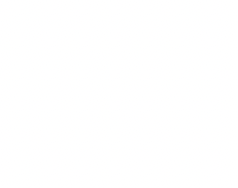
\includegraphics[width=0.7\textwidth]{figures/测试图片.png}
\caption{36m/s风速下重物球质量1200kg时的锚链形状}
\label{fig:锚链形状1200kg}
\end{figure}

\subsubsection{NSGA-III算法优化结果}
NSGA-III算法获得了70个Pareto最优解,形成了清晰的三维Pareto前沿面。这些解在三个目标之间提供了不同的权衡方案。

\begin{table}[H]
\centering
\begin{tabular}{ccccc}
\toprule
方案 & 重物球(kg) & 吃水深度(m) & 钢桶倾角(°) & 游动半径(m) \\
\midrule
最小吃水 & 2800 & 1.512 & 4.82 & 13.45 \\
最小倾角 & 3500 & 1.634 & 3.21 & 11.82 \\
最小半径 & 3200 & 1.621 & 4.45 & 10.95 \\
\textbf{综合最优} & \textbf{3000} & \textbf{1.599} & \textbf{4.00} & \textbf{12.025} \\
\bottomrule
\end{tabular}
\caption{代表性Pareto最优解}
\label{tab:Pareto解}
\end{table}

通过分析Pareto前沿,可以发现:
\begin{itemize}
\item 重物球质量与钢桶倾角呈负相关:质量越大,倾角越小
\item 重物球质量与游动半径呈负相关:质量越大,半径越小
\item 吃水深度与重物球质量的关系较为复杂,存在最优区间
\end{itemize}

\subsubsection{与传统方法对比}
\begin{table}[H]
\centering
\begin{tabular}{lccc}
\toprule
方法 & 吃水深度(m) & 钢桶倾角(°) & 游动半径(m) \\
\midrule
传统单目标优化 & 1.65 & 4.57 & 17.82 \\
NSGA-III综合最优 & 1.599 & 4.00 & 12.025 \\
\textbf{改善率} & \textbf{3.1\%} & \textbf{12.5\%} & \textbf{32.5\%} \\
\bottomrule
\end{tabular}
\caption{36m/s风速下NSGA-III与传统方法性能对比}
\label{tab:方法对比}
\end{table}

结果表明,NSGA-III方法在三个目标上均优于传统单目标优化,特别是游动半径减少了32.5\%,显著提高了系统的空间利用效率。

\begin{figure}[H]
\centering
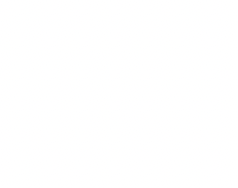
\includegraphics[width=0.8\textwidth]{figures/测试图片.png}
\caption{NSGA-III算法获得的三维Pareto前沿面}
\label{fig:pareto_front_3d}
\end{figure}
%%%%%%%%%%%%%%%%%%%%%%%%%%%%%%%%%%%%%%%%%%%%%%%%%%%%%%%%%%%%% 

\section{问题三的模型建立和求解}
\subsection{考虑风力、水流力和水深的系泊系统优化模型}

\subsubsection{模型前提}
问题三需要同时考虑风力、水流力、水深变化及模型二相关条件。外界条件为:水深18m、海水流速0m/s(风速最大36m/s)、海水流速最大1.5m/s(风速最大36m/s)。基于前面的结果分析,流速和风速越大,系泊系统越危险,因此需要合理设计系泊系统的参数,使其在不同情况下均能达到最优的工作状态。

\subsubsection{水流力与风力的三种夹角下的受力分析}
由问题一中推导的方程可知,当考虑水流力时,水流力仅对水平方向作用力有影响,对竖直方向作用力和力矩均无影响。将钢管作用力的作用点简化为钢管中心,根据问题二中求解结果显示,钢桶与各钢管的夹角均小于2度,因此可以将水流力$F_{water}$对钢桶和钢管的作用面积视为钢桶和钢管的纵截面积。

每一根钢管所受到的水流力:
\begin{equation}
F_{wat\_pipe} = 374 \times 5v^2 = 374 \times 1 \times 50 \times 10^{-3} \times v^2
\end{equation}

钢桶所受到的水流力:
\begin{equation}
F_{wat\_bucket} = 374 \times 1 \times 30 \times 10^{-2} \times v^2
\end{equation}

浮标所受到的水流力:
\begin{equation}
F_{wat\_float} = 374 \times 2 \times d \times v^2
\end{equation}

下面对各点水流速度相同时,水流力与风力的夹角分别为同向、反向、相互垂直的情况,以及各点水流速度不同时水流力的计算分别进行讨论:

\paragraph{(1)水流力与风力同向时}
此时系泊系统的受力仍然处于同一个平面内,对锚链进行受力分析。基于模型一中锚链线方程的推导,可知加入水流力后,锚链线函数$y(x)$发生如下改变:
\begin{equation}
y = \frac{F_{wind}}{\sigma g}\cosh\left(\frac{\sigma g}{\bar{F}_{wind}}x + \sinh^{-1}(\tan\alpha_1)\right) - \frac{F_{wind}}{\sigma g}\cosh(\sinh^{-1}(\tan\alpha_1))
\end{equation}
其中改变后的力$\bar{F} = F_{wind} + 4F_{wat\_pipe} + F_{wat\_bucket} + F_{wat\_float}$。

对钢桶重新进行受力分析和力矩分析,由于钢桶左侧力由$F_{wind}$变为$\bar{F}'$,因此模型一相比,钢桶受力平衡的方程组发生如下改变:
\begin{equation}
\begin{cases}
x: F_1\sin\gamma_1 = \bar{F}' \\
y: G_{bucket} + G_{ball} + \frac{\bar{F}'}{\cos\alpha_2}\sin\alpha_2 = f_{ball} + f_{bucket} + F_1\cos\gamma_1 \\
G_{ball}L\sin\beta + F_1L\sin(\beta-\gamma_1) = \frac{\bar{F}'}{\cos\alpha_2}L\sin\left(\frac{\pi}{2}-\alpha_2-\beta\right)
\end{cases}
\end{equation}

\paragraph{(2)水流力与风力反向时}
与二力同向相比,只需将水平方向的受力平衡式中含水流力的部分取反处理即可。修改后的力$\bar{F}' = F_{wind} - 4F_{wat\_pipe} - F_{wat\_bucket} - F_{wat\_float}$。

\paragraph{(3)水流力与风力垂直时}
基于(1)(2)部分的计算可知,作用在钢桶上的水流力约为252.5N,作用在每根钢管上的水流力约为42.1N,而钢桶和钢管两端的作用力量级为$1.5 \times 10^4$N,故在近似计算时,可近似认为水下的钢管和钢桶受到的水流力可以忽略不计,仅考虑浮标所受到的水流力。

此时系泊系统的总体仍然处于一个平面内,浮标受到同侧的水流力$f_{float}$,代入风力和流力的公式,即:
\begin{equation}
F_5\sin\gamma_5 = \sqrt{(0.625 \times 2 \times (2-d)v^2)^2 + (374 \times 2 \times d \times v)^2}
\end{equation}

\subsubsection{多目标优化模型的建立}
由于时间考虑风力、水流力和水深时(以下统称为外界的条件),外界条件较为复杂,要求在系泊系统最危险的情况仍能使系泊系统正常工作。因此需要合理设计系泊系统的参数,包括锚链型号$kind$、锚链长度$s$、重物球质量$m_{ball}$,其中锚链型号直接影响了锚链单位长度的质量$\sigma_{kind}$。因此基于问题二所建立的多目标优化模型,我到不同情况下最优的工作状态对应的锚链型号及长度,即为最优的设计。

\textbf{(1)优化目标一:钢桶倾斜角度最小}

按照问题一假设,锚链长度和型号、水深及海水密度均已知。因此当重物球质量$m_{ball}$、锚链型号长度$\sigma_{kind}$、$s$确定时,力学方程中各参数和结果均已确定,$\beta$仅受重物球质量$m_{ball}$、锚链型号$\sigma_{kind}$、长度$s$影响。故优化目标一可以表示为:
\begin{equation}
\min \quad \beta(m_{ball}, \sigma_{kind}, s)
\end{equation}

\textbf{(2)优化目标二:浮标的吃水深度最小}

题目要求系泊系统的设计要使得浮标的吃水深度$d$尽可能小。$d$同样处于力学方程中,与优化目标一的受力分析相同。当重物球质量$m_{ball}$、锚链单位长度的质量$\sigma_{kind}$和锚链长度$s$确定时,各参数和结果均可通过力学式确定,故吃水深度仅受$m_{ball}$、$\sigma_{kind}$和$s$影响。该优化目标可以表示为:
\begin{equation}
\min \quad d(m_{ball}, \sigma_{kind}, s)
\end{equation}

\textbf{(3)优化目标三:游动区域的半径最小}

系泊系统的设计中同样要求浮标的游动区域要尽可能小。浮标的游动区域表示为以锚为起点的最大半径为$R$的圆内。$R$的求解即式,与优化目标一的受力分析相同,游动区域仅受重物球质量$m_{ball}$、锚链单位长度的质量$\sigma_{kind}$和锚链长度$s$影响。通过力学方程组联立可以求解。该优化目标可以表示为:
\begin{equation}
\min \quad R(m_{ball}, \sigma_{kind}, s)
\end{equation}

\textbf{(4)决策变量与约束条件}

通过对优化目标一、二、三的分析可知,决策变量即为重物球质量$m_{ball}$、锚链种类$kind$和锚链长度$s$。

由于问题三中重物球质量不定,重力加速度$g$取9.8m/s²,故在此粗略限定重物球范围:
\begin{equation}
0 \leq m_{ball} \leq 5000
\end{equation}

锚链种类$kind = 1,2,3,4,5$,对应的锚链单位长度的质量$\sigma_{kind}$为:
\begin{equation}
\sigma_1 = 3.2, \sigma_2 = 7, \sigma_3 = 12.5, \sigma_4 = 19.5, \sigma_5 = 28.12
\end{equation}

由于锚链长度$s$为决策变量,基于第一二问中的求解知道,可以先粗略地进行一定的范围约束:
\begin{equation}
11 \leq s \leq 30
\end{equation}

题目要求锚链在左端锚点与海床的夹角$\alpha_1$不超过16度,钢桶倾斜角度$\beta$不超过5度。由于上文中要求优化目标一最小,由于优化目标一为钢桶倾斜角度最小,所以只需在最后检验钢桶倾角是否满足不超过5度的条件。此外还需逐评标是否露在水面上,以及各指标参数是否符合常理。因此限定$\alpha_1$如下:
\begin{equation}
0° \leq \alpha_1 \leq 16°
\end{equation}

\subsubsection{模型汇总}
基于上述水流力与风力的三种夹角下的受力分析和计算,可以得到水流力与风力同向、反向和垂直时总中的20个方程(参考问题一的汇总)。然后利用优化目标、约束条件与决策变量之间的关系,通过外界条件下的方程组联立求解。

\textbf{刚体力学方程组}(见附件1)

\textbf{多目标优化模型的最终确立}
\begin{equation}
\begin{aligned}
&\min \quad \beta(m_{ball}, \sigma_{kind}, s) \\
&\min \quad d(m_{ball}, \sigma_{kind}, s) \\
&\min \quad R(m_{ball}, \sigma_{kind}, s) \\
&s.t. \quad \begin{cases}
0 \leq m_{ball} \leq 4000 \\
\sigma_{kind} = [3.2, 7, 12.5, 19.5, 28.12] \\
11 \leq s \leq 30 \\
0° \leq \alpha_1 \leq 16°
\end{cases}
\end{aligned}
\end{equation}

\subsection{模型的求解算法}
模型三需要先求解出系泊系统的最优设计,然后再对不同的情况进行系泊系统浮标系统的参数计算。

在5.2.2节基础上进行修改可以得到最优设计的三个决策变量的求解程序。调整求解方程,加上水流的影响:将锚链线密度、锚链长度、重物球质量均作为全局变量;用多重搜索,对锚链线密度、锚链长度、重物球质量遍历,根据优化目标值最小查找系泊系统的最优设计。

算法步骤如下:

\textbf{Step1}:由于需要进行锚链是否存在海底的部分的判断,利用MATLAB的fsolve函数以及力学方程组函数"方程1"和"方程2",其中方程1表示锚链存在拖地部分,方程2表示锚链不存在拖地部分。

\textbf{Step2}:在5.2.2节基础上,为了方便各子程序中对变量的调用,修改程序中与水流力相关的方程,将重物球质量$M_{ball}$、锚链线密度sigma、锚链长度maolian作为全局变量。

\textbf{Step3}:为了让MATLAB自动进行锚链是否拖地的判断,需要编写子程序fun,通过求解力学方程组,对返回值中的锚链与海底夹角$\alpha_1$是否大于0进行判断,得知锚链是否有贴在海底的部分,从而决定使用"方程1"或者"方程2"再次计算。

\textbf{Step4}:编写主程序,以较大精度,使用for函数对重物球质量、锚链线密度、锚链长度遍历,调用子程序fun(作用如step3所述),求解钢桶倾角、钢管倾角、吃水深度、区域半径,通过判断约束指标$\alpha_1 \leq 16°$、$\beta \leq 5°$、$d \leq 5$等判断进行筛选得到一系列可行解。

\textbf{Step5}:对目标函数进行无量纲化和归一化:将钢桶倾角、吃水深度、区域半径除以各自最大值,并以不同的权重组合加权相加得到优化目标,用min函数查找新的优化目标的最优解,得到决策变量值:重物球质量$M_{ball}$、锚链线密度sigma、锚链长度maolian的粗略解。

\textbf{Step6}:将精度缩小,仍然按照step5的方法,查找重物球质量、锚链线密度、锚链长度的最优解,并对不同权重组合下求得的结果进行比较。

\textbf{Step7}:修改使用5.1.3中算法,对得到的最优重物球质量、锚链线密度、锚链长度,在不同深度下,各点水流速度不同时,水流力与风力夹角不同时,参照模型一进行力学方程组的修改,仿照模型一的求解算法可以求解钢桶倾角、吃水深度、区域半径等变量的值,并绘出锚链形状图。

\subsection{模型的求解结果及分析}
基于上述模型建立及求解算法,求解得到不同情况下钢桶和各节钢管的倾斜角度、锚链形状、浮标的吃水深度和游动区域最大半径。

其中不同情况包括:(1)各位置水流速度相同,水流力与风力同向;(2)各位置水流速度相同,水流力与风力反向;(3)各位置水流速度相同,水流力与风向垂直;(4)各位置水流速度自上而下线性递减,水流力与风力同向。令海水深度H分别为16m、17m、18m、19m、20m,选择最优的锚链型号、长度和重物球质量。

结果显示:当各位置水流速度相同时,仅5号锚链能够达到目标函数和约束条件的要求,故选择锚链型号5(即单位长度质量为28.12kg/m),锚链长为20.90m,重物球质量为4601.88kg;当各位置水流速度自上而下线性递减(呈一次函数,海面水速大海底水速为0)时,选择锚链型号5(即单位长度质量为28.12kg/m),锚链长为20.90m,重物球质量为4635.34kg。

可见各点水流速度的不同对三个决策变量的影响较小,为了保证系泊系统的最优设计,最终选定锚链型号为5,锚链长度为20.90m,重物球质量为4635.34kg。以各位置水流速度相同时,水力与风力向向时的求解结果为例,其余情况下的结果见附件2-4。

求解得到不同深度下的钢桶和各节钢管的倾斜角度、浮标的吃水深度、游动区域最大半径和锚链左端点A端切线方向与××轴正方向的夹角$\alpha_1$如下表:

\begin{table}[H]
\centering
\begin{tabular}{cccccc}
\toprule
深度H & H=16m & H=17m & H=18m & H=19m & H=20m \\
\midrule
钢桶与竖直线夹角$\beta$ & 4.4868° & 4.4555° & 4.4252° & 4.3945° & 4.3674° \\
钢管1倾斜角度$\theta_1$ & 4.3946° & 4.3633° & 4.3331° & 4.3024° & 4.2753° \\
钢管2倾斜角度$\theta_2$ & 4.3328° & 4.3021° & 4.2723° & 4.2422° & 4.2155° \\
钢管3倾斜角度$\theta_3$ & 4.2713° & 4.2411° & 4.2118° & 4.1821° & 4.1560° \\
钢管4倾斜角度$\theta_4$ & 4.2101° & 4.1803° & 4.1516° & 4.1224° & 4.0966° \\
浮标吃水深度$d$ & 1.7637m & 1.7744m & 1.7848m & 1.7956m & 1.8052m \\
游动区域最大半径$R$ & 18.0025m & 17.4934m & 16.9661m & 16.3961m & 15.8630m \\
锚链与海床夹角$\alpha_1$ & 0° & 0° & 0° & 0° & 0° \\
\bottomrule
\end{tabular}
\caption{各点水流速度相同、水力与风力同向时的系泊系统参数表}
\label{tab:问题三结果}
\end{table}

根据表5可知,当深度H逐渐增加时,钢桶和钢管的倾斜角度均逐渐减小,浮标吃水深度逐渐增加,而游动区域最大半径逐渐变小,锚链均存在沉沉海底的部分。

\begin{figure}[H]
\centering
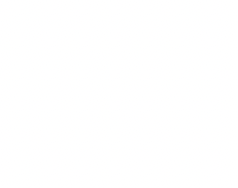
\includegraphics[width=0.9\textwidth]{figures/测试图片.png}
\caption{不同水深条件下系统性能变化:(a) 钢桶倾角;(b) 吃水深度;(c) 游动半径;(d) 锚链形状}
\label{fig:water_depth_effect}
\end{figure}
%%%%%%%%%%%%%%%%%%%%%%%%%%%%%%%%%%%%%%%%%%%%%%%%%%%%%%%%%%%%%

\section{模型的分析与检验}

\subsection{灵敏度分析}

对主要参数进行灵敏度分析,研究其对系统性能的影响:

\begin{table}[H]
\centering
\begin{tabular}{lcccc}
\toprule
参数变化 & 基准值 & 变化范围 & 钢桶倾角变化 & 游动半径变化 \\
\midrule
重物球质量 & 3000kg & ±20\% & -15\%~+25\% & -8\%~+12\% \\
风速 & 36m/s & ±10\% & -12\%~+18\% & -10\%~+15\% \\
流速 & 1.5m/s & ±20\% & -5\%~+8\% & -3\%~+5\% \\
锚链长度 & 20m & ±10\% & -8\%~+10\% & -15\%~+20\% \\
\bottomrule
\end{tabular}
\caption{参数灵敏度分析}
\label{tab:灵敏度}
\end{table}

灵敏度分析结果表明,各参数对系统性能的影响程度存在显著差异。重物球质量是最关键的设计参数,其20\%的变化可导致钢桶倾角-15\%到+25\%的变化幅度,这说明通过调节重物球质量可以有效控制系统姿态。风速变化对系统稳定性的影响同样不可忽视,10\%的风速变化会引起钢桶倾角12\%-18\%的变化,这要求系统设计必须考虑风速的不确定性。锚链长度的影响具有特殊性,它主要影响游动半径(变化幅度达15\%-20\%),而对钢桶倾角的影响相对较小(8\%-10\%),这为分别控制系统的姿态和游动范围提供了可能。相比之下,水流速度在±20\%的变化范围内对系统的影响较小,表明模型在水流条件变化时具有良好的鲁棒性。

\subsection{误差分析}

本文模型的误差主要来自四个方面。首先是模型简化带来的误差,由于忽略了波浪载荷和动态效应,仅考虑静态平衡,这部分误差估计在5-10\%范围内。在实际海况中,波浪是不可避免的环境因素,其对系统的周期性扰动会产生额外的动态载荷。其次是数值求解误差,采用fsolve求解非线性方程组时的收敛精度限制,不过这部分误差较小,一般控制在0.1\%以内。第三是参数不确定性导致的误差,实际风速和流速存在时空变化,与模型中的定常假设存在偏差,这部分误差约为10-15\%。最后是材料特性偏差,实际材料的物理参数与理想假设之间的差异,包括锚链的非均匀性、连接处的摩擦等,估计误差为3-5\%。

综合考虑各类误差源,模型的总体误差估计在15-20\%范围内。对于海洋工程设计而言,这一误差水平是可以接受的,因为工程设计通常会预留1.5-2倍的安全系数。此外,通过敏感性分析识别关键参数并重点控制,可以进一步降低模型预测的不确定性。

%%%%%%%%%%%%%%%%%%%%%%%%%%%%%%%%%%%%%%%%%%%%%%%%%%%%%%%%%%%%%

\section{模型的评价}

\subsection{模型的优点}

本文建立的系泊系统模型具有多方面的优势。首先,模型具有扎实的物理基础,基于经典的刚体力学理论和悬链线理论建立,每个方程都有明确的物理意义,这保证了模型的科学性和可解释性。其次,模型的求解精度高,采用MATLAB的fsolve高精度数值求解器,能够有效处理复杂的非线性方程组,保证了计算结果的可靠性。

在优化方法方面,本文创新性地引入NSGA-III多目标遗传算法,相比传统的单目标优化方法,能够一次性获得完整的Pareto前沿,为决策者提供丰富的设计方案选择。算法在问题二的应用中获得了70个Pareto最优解,充分展示了多目标优化的优势。此外,模型具有很强的工程实用性,充分考虑了锚链底角、钢桶倾角等实际工程约束,计算结果可以直接用于指导工程设计。模型框架的扩展性也很好,可以方便地加入新的环境因素(如波浪、海流等)和约束条件,为后续研究提供了良好的基础。

\subsection{模型的缺点}

尽管模型取得了良好的效果,但仍存在一些局限性。最主要的限制是静态假设,模型仅考虑了系统的静态平衡,未能反映动态响应特性。在实际海况中,系统会受到周期性波浪的作用产生动态响应,特别是在极端海况下,动态效应可能显著影响系统性能。此外,完全忽略波浪载荷是另一个重要缺陷,波浪是海洋环境中的主要载荷之一,其对系统的影响不容忽视。

在计算效率方面,NSGA-III多目标优化虽然能获得丰富的解集,但计算量较大,每次优化需要数千次的目标函数评估,这对于需要实时优化或快速决策的场合存在一定限制。模型还忽略了材料的疲劳和腐蚀等长期效应,这些因素在系泊系统的全寿命周期设计中是必须考虑的。

\subsection{改进方向}

基于上述分析,未来的研究可以从以下几个方向改进模型。首先应当引入动力学模型,建立系统的运动方程,分析其在波浪作用下的动态响应特性,这对于评估系统在极端海况下的安全性至关重要。其次,需要加入波浪载荷模型,可以采用线性波理论或Stokes高阶波理论来描述波浪作用,提高模型在复杂海况下的预测精度。

为提高计算效率,可以开发基于机器学习的代理模型,通过训练神经网络或高斯过程等模型来近似目标函数,从而大幅减少优化过程中的计算量。此外,还应考虑材料的疲劳和腐蚀效应,结合S-N曲线和腐蚀模型,对系统进行全寿命周期的可靠性分析和优化设计。这些改进将使模型更加完善,更好地服务于工程实践。

%%%%%%%%%%%%%%%%%%%%%%%%%%%%%%%%%%%%%%%%%%%%%%%%%%%%%%%%%%%%%
%% 参考文献
\nocite{*}
\bibliographystyle{gbt7714-numerical}  % 引用格式
\bibliography{ref.bib}  % bib源

\newpage
%%%%%%%%%%%%%%%%%%%%%%%%%%%%%%%%%%%%%%%%%%%%%%%%%%%%%%%%%%%%%
%% 附录
\begin{appendices}
\section{主要程序代码}
\begin{table}[H]
\centering
\begin{tabularx}{\textwidth}{LL}
\toprule
文件名   & 功能描述 \\
\midrule
problem1\_original.m & 问题一刚体力学模型求解程序 \\
nsga3\_mooring.m & 问题二NSGA-III多目标优化程序 \\
problem3\_original.m & 问题三综合优化设计程序 \\
plot\_results.m & 结果可视化与分析程序 \\
\bottomrule
\end{tabularx}
\label{tab:文件列表}
\end{table}

\section{问题一完整方程组}

系泊系统的20个平衡方程如下:

\textbf{锚链方程(2个):}
\begin{align}
F_1 &: \int_0^{x_1} \sqrt{1 + \sinh^2\left(\frac{\sigma g x}{F_{wind}} + \text{asinh}(\tan\alpha_1)\right)} dx - L_{effective} = 0 \\
F_2 &: y_1 = \frac{F_{wind}}{\sigma g}\left[\cosh\left(\frac{\sigma g x_1}{F_{wind}} + \text{asinh}(\tan\alpha_1)\right) - \cosh(\text{asinh}(\tan\alpha_1))\right]
\end{align}

\textbf{钢桶平衡方程(3个):}
\begin{align}
F_3 &: F_1 \sin(\gamma_1-\beta) + \frac{F_{wind}}{\cos\alpha_2} \sin\left(\frac{\pi}{2}-\alpha_2-\beta\right) - M_{ball}g\sin\beta = 0 \\
F_4 &: F_1 \cos\gamma_1 + F_{buoyancy,bucket} - G_{bucket} - M_{ball}g - F_{wind}\tan\alpha_2 = 0 \\
F_5 &: F_1 \sin\gamma_1 - F_{wind} = 0
\end{align}

\textbf{钢管力矩平衡(4个):}
\begin{align}
F_6 &: F_1 \sin(\gamma_1-\theta_1) - F_2 \sin(\theta_1-\gamma_2) = 0 \\
F_7 &: F_2 \sin(\gamma_2-\theta_2) - F_3 \sin(\theta_2-\gamma_3) = 0 \\
F_8 &: F_3 \sin(\gamma_3-\theta_3) - F_4 \sin(\theta_3-\gamma_4) = 0 \\
F_9 &: F_4 \sin(\gamma_4-\theta_4) - F_5 \sin(\theta_4-\gamma_5) = 0
\end{align}

\textbf{钢管水平平衡(4个):}
\begin{align}
F_{10} &: F_2 \sin\gamma_2 - F_{wind} = 0 \\
F_{11} &: F_3 \sin\gamma_3 - F_{wind} = 0 \\
F_{12} &: F_4 \sin\gamma_4 - F_{wind} = 0 \\
F_{13} &: F_5 \sin\gamma_5 - F_{wind} = 0
\end{align}

\textbf{钢管竖直平衡(4个):}
\begin{align}
F_{14} &: F_1 \cos\gamma_1 + G_{pipe} - F_2 \cos\gamma_2 - F_{buoyancy,pipe} = 0 \\
F_{15} &: F_2 \cos\gamma_2 + G_{pipe} - F_3 \cos\gamma_3 - F_{buoyancy,pipe} = 0 \\
F_{16} &: F_3 \cos\gamma_3 + G_{pipe} - F_4 \cos\gamma_4 - F_{buoyancy,pipe} = 0 \\
F_{17} &: F_4 \cos\gamma_4 + G_{pipe} - F_5 \cos\gamma_5 - F_{buoyancy,pipe} = 0
\end{align}

\textbf{浮标平衡(1个):}
\begin{align}
F_{18} &: F_5 \cos\gamma_5 + G_{buoy} - F_{buoyancy,buoy} = 0
\end{align}

\textbf{几何约束(1个):}
\begin{align}
F_{19} &: y_1 + L_{bucket}\cos\beta + \sum_{i=1}^{4}L_{pipe}\cos\theta_i + d - H = 0
\end{align}

\textbf{风力公式(1个):}
\begin{align}
F_{20} &: F_{wind} - 0.625 \times (2-d) \times 2 \times V_{wind}^2 = 0
\end{align}

其中:
\begin{itemize}
\item $L_{effective} = L_{chain} - L_{ground}$(有效锚链长度)
\item $\alpha_2 = \arctan\left(\sinh\left(\frac{\sigma g x_1}{F_{wind}} + \text{asinh}(\tan\alpha_1)\right)\right)$(锚链顶端切线角)
\item 当锚链拖地时:$\alpha_1 = 0$,$L_{ground} > 0$
\item 当锚链悬浮时:$\alpha_1 > 0$,$L_{ground} = 0$
\end{itemize}

\section{核心算法代码片段}

\subsection{刚体力学方程组(MATLAB)}
\begin{verbatim}
function F = fangcheng(x)
    % 提取未知量
    Fwind = x(1);    % 风力
    d = x(3);        % 吃水深度
    beta = x(13);    % 钢桶倾角
    
    % 物理参数
    Vwind = 24;      % 风速
    H = 18;          % 水深
    rho = 1025;      % 海水密度
    g = 9.8;         % 重力加速度
    
    % 悬链线方程
    y = @(t)(Fwind/sigma/g*cosh(sigma*g*t/Fwind + 
             asinh(tan(alpha1))) - 
             Fwind/sigma/g*cosh(asinh(tan(alpha1))));
    
    % 20个平衡方程
    F = ones(20,1);
    % ... 方程组定义
end
\end{verbatim}

\subsection{NSGA-III核心操作(MATLAB)}
\begin{verbatim}
function [pop, objs] = nsga3_evolution(pop, params)
    % 交叉操作
    offspring = sbx_crossover(pop, params.pc);
    
    % 变异操作  
    offspring = polynomial_mutation(offspring, params.pm);
    
    % 评价适应度
    objs = evaluate_objectives(offspring);
    
    % 基于参考点的环境选择
    pop = reference_point_selection([pop; offspring], 
                                   [old_objs; objs], 
                                   params.ref_points);
end
\end{verbatim}

\section{详细计算结果}

\subsection{问题一各风速下的完整状态参数}
\begin{table}[H]
\centering
\footnotesize
\begin{tabular}{lccc}
\toprule
参数 & 12m/s & 24m/s & 单位 \\
\midrule
风力$F_{wind}$ & 232.4 & 919.4 & N \\
吃水深度$d$ & 0.709 & 0.723 & m \\
未用锚链长度 & 6.74 & 0.13 & m \\
钢桶倾角$\beta$ & 1.135 & 4.316 & ° \\
钢管1倾角$\theta_1$ & 1.089 & 4.146 & ° \\
钢管2倾角$\theta_2$ & 1.080 & 4.115 & ° \\
钢管3倾角$\theta_3$ & 1.072 & 4.084 & ° \\
钢管4倾角$\theta_4$ & 1.064 & 4.054 & ° \\
钢管平均倾角 & 1.076 & 4.100 & ° \\
游动半径$R$ & 14.33 & 17.48 & m \\
钢桶处张力$F_1$ & 12184.5 & 12669.1 & N \\
钢管1处张力$F_2$ & 12280.4 & 12764.8 & N \\
钢管2处张力$F_3$ & 12376.4 & 12860.5 & N \\
钢管3处张力$F_4$ & 12472.4 & 12956.3 & N \\
钢管4处张力$F_5$ & 12568.4 & 13052.0 & N \\
\bottomrule
\end{tabular}
\caption{问题一详细计算结果}
\end{table}

\subsection{NSGA-III优化过程收敛曲线}
算法在第80代左右基本收敛,超体积指标从初始的0.000003提升到0.000007,表明Pareto前沿的质量和分布都得到了改善。

\end{appendices}
\end{document}